\section{Introduction}
\label{sec:introduction}

Reinforcement learning (RL) has become an essential method for post-training frontier large language models (LLMs), enhancing their reasoning, math, and agentic capabilities~\citep{guo2025deepseek, yang2025qwen3, team2025kimi, zeng2025glm}.
Among RL algorithms, on-policy RL collects rollouts from the same policy being optimized, reducing policy-staleness degradation and improving training stability and model quality~\citep{kumar2025llm,fu2025areal}.
However, rollout generation has emerged as the dominant \bottleneck{} in the RL pipeline because post-trained models increasingly generate long responses~\citep{chen2024not,guo2025deepseek,yu2025dapo,liu2025understanding} that must be decoded token by token.
Consequently, reducing rollout latency is critical for accelerating RL post-training, since it often dominates other parallelizable stages such as policy updates~\citep{schulman2017proximal}.

Speculative decoding (SD)~\citep{leviathan2023fast,chen2023accelerating} offers a promising way to reduce inference latency while preserving the policy distribution.
SD uses a cheaper drafter to propose multiple candidate tokens, which are then verified in parallel by the target model, \textit{i.e.}, the policy being sampled.
Its speedup depends on two conditions: algorithmically, the block efficiency $\mal$ must be sufficiently high, where $\mal$ measures how many target-distributed tokens each draft-verify iteration produces on average~\citep{zhou2024distillspec,liu2025speculative};
system-wise, decoding should not be pushed into a compute-bound regime, so that parallel target-model verification can exploit underutilized compute~\citep{leviathan2023fast,sadhukhan2024magicdec,liu2025speculative}.

\begin{figure*}[t]
    \centering
    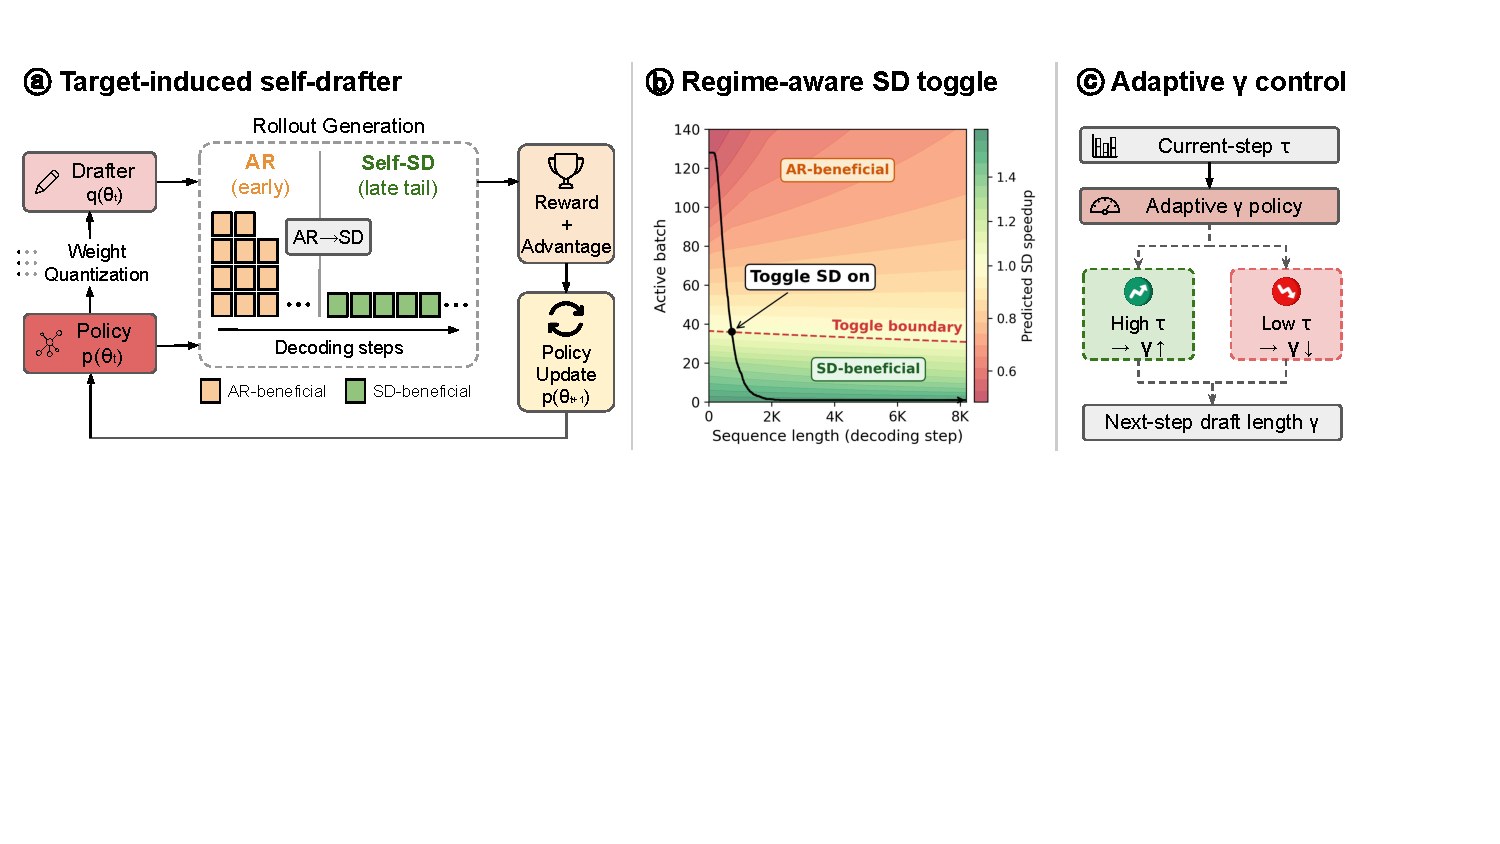
\includegraphics[width=\textwidth]{figures/main_teaser.pdf}
    \caption{
    \textbf{Overview of \methodtitle{}}.
    \methodtitle{} bridges the gap between SD for fixed-model serving and RL rollout decoding through three coordinated components:
    (a) per-step self-drafter refresh to track the evolving policy,
    (b) regime-aware toggling from AR to SD under tail-heavy rollout dynamics (see~\cref{fig:rollout_bottleneck_appendix}), and
    (c) adaptive draft length $\gamma$ control based on observed block efficiency $\tau$.
    }
    \label{fig:main_teaser}
\end{figure*}

In this regard, RL introduces challenges absent from serving fixed LLMs, making existing SD methods nontrivial to apply to RL rollouts.
First, the target policy continuously evolves during training, making static drafters stale and potentially reducing block efficiency~\citep{zhang2025fastgrpo}.
Second, rollout generation often starts with large active batch sizes, creating compute-bound intervals where SD may be slower than autoregressive (AR) decoding, before the batch later shrinks as shorter responses finish.
At the same time, RL creates an opportunity: as post-training sharpens the policy distribution~\citep{zhao2025echo}, the target policy can be approximated by a lower-capacity subset induced from the target itself, which can still cover the concentrated probability mass.
Together, these factors raise a practical question: \emph{how can SD realize speedup in RL rollouts under the distinct conditions introduced by RL?}

Prior SD methods for RL rollouts address this problem, but still face either low block efficiency or the burden of drafter construction and adaptation.
\History{} methods reuse previous-epoch rollouts as draft proposals and are easy to deploy, but their low-capacity drafters often yield limited block efficiency because past rollouts sparsely cover future trajectories~\citep{liu2025spec,he2025history,shao2025beat}.
\Learned{} methods seek higher block efficiency by training auxiliary drafters, but existing learned auxiliary drafters do not automatically align with RL rollout distributions; in practice, they often require separate drafter pretraining and continual online adaptation to track the evolving target policy, adding training overhead and system complexity~\citep{zhang2025fastgrpo,chen2025respec,hu2026taming}.
% \mj{\rev{move the question into the end of the previous paragraph?; Can we transfer the realized speedup from ... to ... while ...}}This raises a central question: \emph{Can speculative decoding deliver realized rollout speedup while maintaining high block efficiency without an additional pipeline for drafter pretraining and adaptation?}


To this end, we answer this question with \textbf{\methodtitle}, a system-aware SD framework designed for on-policy RL rollouts~(\cref{fig:main_teaser}).
We first characterize rollout workloads, showing that target-induced drafters naturally stay coupled to the evolving policy and that dense weight projections dominate tail decoding.
Based on these observations, we induce a weight-quantized drafter from the current target policy at every training step, achieving high block efficiency without separate drafter pretraining or online drafter updates.
We further introduce two control policies: a system-aware SD toggle that activates SD only in favorable regimes, avoiding slowdowns during early compute-bound large-batch phases, and an adaptive draft-length policy that matches the drafting budget to evolving acceptance behavior during RL.
We show that \methodtitle{} reduces rollout and end-to-end latency by up to~\speeduprollout{} and~\speedupete{}, respectively, over prevalent RL training and serving stacks~\citep{sheng2025hybridflow,kwon2023efficient}.

Our main contributions are as follows:

\begin{itemize}[leftmargin=*]
\item We characterize SD for RL rollouts, showing how evolving policies, shrinking-batch dynamics, and rollout-tail latency motivate a system-aware self-SD design~(\cref{sec:preliminary}).
\item We present \methodtitle{}, an RL-specific SD framework with a target-induced quantized drafter, dynamic SD toggling, and adaptive drafting budgets~(\cref{sec:method}).
\item We show that \methodtitle{} reduces rollout and end-to-end latency by up to~\speeduprollout{} and~\speedupete{} over a standard accelerated AR rollout baseline~\citep{sheng2025hybridflow,kwon2023efficient}, and analyze why existing SD approaches do not consistently resolve the emergent challenges of RL rollouts~(\cref{sec:Evaluation}).
\end{itemize}
